\chapter{Requirements, Methodology, and Project Management}
\begin{spacing}{1.2}
\minitoc
\thispagestyle{MyStyle}
\end{spacing}
\newpage

\section*{INTRODUCTION}
\addcontentsline{toc}{section}{INTRODUCTION}
Chapter~1 established the audit findings and the strategic pivot they produced; Chapter~2 positioned the proposed platform against existing approaches. This chapter formalises the engineering structure that disciplined the work: the stakeholders, actors, and access assumptions that shape the system, the functional and non-functional requirements derived from the audit, the use cases and activity diagrams, and the methodology adopted under the constraints of a solo-developer project.

\section{Stakeholders, Actors, and Access Assumptions}
The platform serves two distinct populations: \textit{stakeholders},
whose expectations frame the project's definition of success, and
\textit{actors}, the roles that interact with Itqan through its user
interfaces, its API, or its conversational layer.

\subsection{Project Stakeholders}
Four stakeholders shape this project: the academic supervisor at
ENET'COM, the professional supervisor at \hostCompany, the technical
and leadership stakeholders at \clientCompany, and the academic jury.

\subsection{System Actors}
The platform's interaction model recognises five actors --- three
currently exercised and two reserved for target functionality beyond
the present scope. Conversational interactions through the RFQ Copilot
are not modelled as a separate actor: the copilot is a cross-cutting
capability exercised by the three current business actors below, with
access scope always tied to the authenticated business role.
Table~\ref{tab:actors} summarises the catalogue.

\begin{table}[H]
\centering
\renewcommand{\arraystretch}{1.4}
\begin{tabularx}{\textwidth}{|p{2.9cm}|>{\RaggedRight\arraybackslash}X|p{1.8cm}|}
\hline
\rowcolor{lightgray}
\textbf{Actor} & \textbf{Role and Responsibilities} & \textbf{Status} \\ \hline
Estimation Manager & Operational control of the RFQ lifecycle: intake, feasibility check, classification, workflow monitoring, stage supervision, and bid approval. Reflects the coordinating role observed in GHI's estimation department. & Current \\ \hline
Estimator & Performs the detailed cost estimation work on assigned RFQs: fills the estimation workbook, attaches artifacts and notes to the relevant lifecycle stages, and advances the RFQ through the estimation phase. & Current \\ \hline
Executive & Consumes portfolio indicators and decision-oriented summaries through analytical endpoints and dashboards, without operating on individual RFQs. & Current \\ \hline
Department User & Consolidated actor reserved to represent the Engineering, Production, Quality, and Procurement contributors identified during the audit (Chapter~1, §1.2), each providing stage-specific inputs and resolving blockers raised against their department. & Future \\ \hline
Administrator & Manages workflow templates and access-management responsibilities once the dedicated identity service is in place. & Future \\ \hline
\end{tabularx}
\caption{System actors of Itqan with their responsibilities and implementation status}
\label{tab:actors}
\end{table}

\subsection{Permission Model and IAM Integration}
Each actor is bound to a permission scope that defines which RFQs are
visible, which lifecycle operations are permitted, and which
analytical surfaces are exposed. Table~\ref{tab:permissions} summarises
the target permission model for the three current actors; the two
future actors inherit additional permissions once the dedicated
identity service is delivered.

\begin{table}[H]
\centering
\renewcommand{\arraystretch}{1.3}
\scriptsize
\begin{tabularx}{\textwidth}{|p{2.5cm}|>{\RaggedRight\arraybackslash}X|>{\RaggedRight\arraybackslash}X|>{\RaggedRight\arraybackslash}X|}
\hline
\rowcolor{lightgray}
\textbf{Actor} & \textbf{Lifecycle Operations} & \textbf{Analytics Surface} & \textbf{Copilot Scope} \\ \hline
Estimation Manager & Full read and write across all RFQs in the department portfolio; classification, approval, and stage supervision authority & Full portfolio analytics & Portfolio mode and RFQ-bound mode across all department RFQs \\ \hline
Estimator & Read and write on assigned RFQs only; advance assigned RFQs through estimation-phase stages & Read-only on personal pipeline indicators & RFQ-bound mode on assigned RFQs; portfolio mode scoped to assigned RFQs \\ \hline
Executive & Read-only on portfolio aggregates; no operations on individual RFQs & Full portfolio analytics and decision-oriented summaries & Portfolio mode only \\ \hline
\end{tabularx}
\caption{Target permission model for currently exercised actors}
\label{tab:permissions}
\end{table}

In the current scope, this permission model is enforced through \textit{actor-context propagation}: every inbound request carries an authenticated actor identity, which the manager service uses to scope retrievals and to authorise stage-changing operations. The copilot inherits this scope rather than holding its own, since every evidence read is routed through the manager service (FR-COP-06, NFR-SEC-02). A future dedicated \textit{Identity and Access Management (IAM) service} is reserved as integration point in the manager (bearer-token path and identity-resolution connector); full cross-user isolation and granular permission management are deferred to that service (NFR-SEC-01, NFR-SEC-04).


\section{Functional Requirements}
The functional requirements of Itqan describe the operational capabilities the platform must offer to the actors of Section~3.1. They are derived directly from the audit findings of Chapter~1 --- each pain point shapes one or more requirements --- and are organised by module, each with a unique identifier referenced in the validation evidence of Chapter~6.

The functional requirements are organised into twenty-five items distributed across the four platform modules and cross-cutting concerns. Eight \textbf{Manager-service} requirements (FR-MGR-01 to FR-MGR-08) cover RFQ registration with classification metadata, workflow-instantiated stage representation, three-gate stage progression (mandatory-field, blocker, transition-validity), artifact attachment with append-only note semantics, manual and rule-based reminder management, analytical aggregations (status totals, win-rate, per-client), lifecycle traceability through non-destructive update semantics, and soft-delete propagation on subtask deletion. Eight \textbf{Copilot-service} requirements (FR-COP-01 to FR-COP-08) cover evidence-grounded natural-language responses, dual portfolio / RFQ-bound entry contexts, deterministic turn classification into a known path, path-authorised evidence grounding (manager state in current scope, intelligence artifacts when their paths ship), structured refusal for out-of-scope queries, manager-mediated access enforcement on every retrieval, bounded working-memory capture, and draft verification against retrieved evidence before delivery. Four \textbf{Intelligence-service} requirements (FR-INT-01 to FR-INT-04) cover MR-package parsing against the canonical section layout, estimation-workbook parsing against the GHI template (three-sheet anchor set: \textit{General}, \textit{Bid~S}, \textit{Top Sheet}), intelligence briefing for downstream presentation, and structured anomaly surfacing rather than silent correction. Three \textbf{User-Interface} requirements (FR-UI-01 to FR-UI-03) cover the portfolio view, the RFQ detail view, and the role-aware executive indicators surface. Two \textbf{Cross-cutting} requirements (FR-X-01, FR-X-02) cover independent backend containerisation and the health/observability endpoint surface.

The full backlog, with priority and current implementation status per item, is reproduced in Appendix~A.2 (Table~\ref{tab:backlog}); current implementation and validation coverage of each requirement are discussed in Chapters~5 and~6.

\subsection{Product Backlog}
The functional requirements above are tracked operationally as a 25-item product backlog, grouped by module and prioritised; the full backlog is reproduced in Appendix~A.2. The single Low-priority item, the dedicated identity service, is deliberately deferred, as established in Chapter~1.

\section{Non-Functional Requirements}
The non-functional requirements span standard production-grade concerns and concerns specific to an LLM-based conversational layer, grouped into five categories: Reliability (REL), Security (SEC), AI Integrity (AI), Maintainability (MNT), and Operability (OPS). Each row carries a Scope/Status tag distinguishing implemented attributes from partial or deferred ones (Table~\ref{tab:nfr}).

\begingroup
\renewcommand{\arraystretch}{1.2}
\scriptsize
\begin{xltabular}{\textwidth}{|p{2.2cm}|p{2.7cm}|>{\RaggedRight\arraybackslash}X|p{2.7cm}|}
\caption{Non-functional requirements grouped by category, each tagged with its current scope and implementation status}
\label{tab:nfr} \\
\hline
\rowcolor{lightgray}
\textbf{ID} & \textbf{Category} & \textbf{Requirement} & \textbf{Scope / Status} \\ \hline
\endfirsthead
\multicolumn{4}{l}{\textit{\tablename~\thetable\ --- continued from previous page}} \\
\hline
\rowcolor{lightgray}
\textbf{ID} & \textbf{Category} & \textbf{Requirement} & \textbf{Scope / Status} \\ \hline
\endhead
\hline
\multicolumn{4}{r}{\textit{continued on next page}} \\
\endfoot
\hline
\endlastfoot
NFR-REL-01 & Reliability & State-changing operations on lifecycle records shall preserve traceability through timestamps and non-destructive update semantics; a dedicated audit-log surface is a hardening direction. & Implemented; audit-log hardening direction \\ \hline
NFR-REL-02 & Reliability & The system shall fail safely on transient infrastructure errors by preserving already persisted state and returning structured errors, so that operations can be safely re-attempted. & Partial; safe-failure implemented, automatic retry deferred \\ \hline
NFR-REL-03 & Reliability & Records configured for soft deletion shall remain available for review; no destructive deletion shall occur on critical lifecycle records. & Implemented \\ \hline
NFR-REL-04 & Reliability & State-changing operations and errors in the manager service shall carry a structured, correlatable request identifier supporting manager-level tracing. & Partial; manager-internal implemented, cross-service deferred \\ \hline
NFR-SEC-01 & Security & Role-based access control shall be enforceable at the service layer independently of the calling client; in current scope this is exercised through actor-context headers and manager-mediated retrieval, with the manager carrying a built IAM integration point and the dedicated identity service deferred. & Partial; IAM integration point built, identity service deferred \\ \hline
NFR-SEC-02 & Security & The copilot service shall not bypass the access controls of the manager service: every retrieval shall be mediated through the manager's authorized endpoints. & Implemented \\ \hline
NFR-SEC-03 & Security & Authentication credentials and external API keys shall not appear in logs, responses, or persisted records. & Implemented as coding discipline; automated redaction test recognised as hardening direction \\ \hline
NFR-SEC-04 & Security & The schema and queries shall be structured so that per-user scoping of retrievals is achievable at the data layer; full enforcement of cross-user data isolation is contingent on the dedicated identity service. & Partial; IAM deferred \\ \hline
NFR-AI-01 & AI Integrity & The copilot shall not produce factual claims about RFQs, lifecycle state, or platform data unsupported by evidence retrieved at the same turn. & Implemented (Path~4) \\ \hline
NFR-AI-02 & AI Integrity & The copilot shall explain its responses with reference to the evidence used, in a form that allows the user to verify the claim. & Implemented (Path~4) \\ \hline
NFR-AI-03 & AI Integrity & The copilot shall refuse, rather than approximate, queries outside its supported scope or lacking sufficient evidence. & Implemented \\ \hline
NFR-AI-04 & AI Integrity & The copilot's authority over operational truth, evidence selection, and access enforcement shall remain owned by deterministic platform components, not the language model. & Implemented \\ \hline
NFR-MNT-01 & Maintainability & Each service shall expose its capabilities through a versioned, documented API contract; internal data structures shall not leak across service boundaries. & Implemented \\ \hline
NFR-MNT-02 & Maintainability & Each backend service shall follow the BACAB layered architecture pattern (routes, controllers, datasources, with translators, models, configuration, and utilities as support layers). & Implemented (backend services) \\ \hline
NFR-MNT-03 & Maintainability & Major architectural decisions shall be captured in a structured Architectural Decision Record format with context, alternatives, and consequences. & Implemented for headline decisions (e.g., ADR-H5); consolidated register file not yet committed to the code repository \\ \hline
NFR-OPS-01 & Operability & The backend services shall be containerized and independently startable, with configuration externalized. & Partial; backend containerized, root composition and UI deferred \\ \hline
NFR-OPS-02 & Operability & Each backend service shall expose a health endpoint; readiness probes and metrics endpoints are provided where implemented. & Partial; /health on all backends, /metrics on manager only, /readiness recognised as hardening direction \\ \hline
NFR-OPS-03 & Operability & The manager service shall emit structured logs including a correlation identifier; structured logging and cross-service correlation propagation on the remaining services are hardening directions. & Partial; manager only, cross-service propagation deferred \\ \hline
NFR-OPS-04 & Operability & Synchronous operational endpoints shall remain compatible with an interactive user experience under nominal validation and demonstration conditions. & Observed in functional testing; no dedicated load-test campaign \\ \hline
\end{xltabular}
\endgroup

\section{Use Cases and Activity Diagrams}
This section presents the behavioural view of Itqan: the use cases through which the actors of Section~3.1 interact with the platform, and the activity flow of the workflow whose internal logic best characterises the project.

\subsection{System-Level Use Case}
Eight use cases structure the interaction surface of Itqan.
Table~\ref{tab:use_case_matrix} presents the actor-use-case
responsibility matrix, summarising which actors exercise each use case
and under what scope.

\begin{table}[H]
\centering
\renewcommand{\arraystretch}{1.3}
\scriptsize
\begin{tabularx}{\textwidth}{|>{\RaggedRight\arraybackslash}X|c|c|c|c|c|}
\hline
\rowcolor{lightgray}
\textbf{Use Case} & \textbf{Manager} & \textbf{Estimator} & \textbf{Executive} & \textbf{Dept. User (future)} & \textbf{Admin (future)} \\ \hline
Consult RFQ Portfolio & ✓ & ✓ (scoped) & ✓ & ✓ & --- \\ \hline
Register RFQ & ✓ & --- & --- & --- & --- \\ \hline
Advance RFQ Stage & ✓ & ✓ (assigned) & --- & ✓ (own stage) & --- \\ \hline
Manage Stage Artifacts & ✓ & ✓ (assigned) & --- & ✓ (own stage) & --- \\ \hline
Configure Reminders & ✓ & ✓ (own) & --- & ✓ (own) & --- \\ \hline
Consult Pipeline Analytics & ✓ & ✓ (limited) & ✓ & --- & --- \\ \hline
Consult the RFQ Copilot & ✓ & ✓ (scoped) & ✓ (portfolio mode) & ✓ & --- \\ \hline
Manage Workflow Templates & --- & --- & --- & --- & ✓ \\ \hline
\end{tabularx}
\caption{Actor-use-case responsibility matrix: rows are use cases, columns are actors, cells indicate access scope}
\label{tab:use_case_matrix}
\end{table}

The use cases are defined as follows. \textit{Consult RFQ Portfolio}
is the entry point for all business actors, returning the list of
RFQs visible under the actor's permission scope. \textit{Register RFQ}
performs intake of a new RFQ with its identifying metadata and
workflow template (FR-MGR-01). \textit{Advance RFQ Stage} progresses
an RFQ through its lifecycle stages, gated by the validation rules of
FR-MGR-03. \textit{Manage Stage Artifacts} attaches files, notes, and
subtasks to a stage, with append-only semantics for notes (FR-MGR-04).
\textit{Configure Reminders} creates and assigns manual or rule-based
reminders against stages or subtasks (FR-MGR-05). \textit{Consult
Pipeline Analytics} exposes portfolio aggregates including status
totals, terminal-outcome win rate, and per-client breakdown
(FR-MGR-06). \textit{Consult the RFQ Copilot} provides conversational
access to platform evidence, with two invocation contexts modelled as
extension points: \textit{portfolio mode}, entered from the home view,
and \textit{RFQ-bound mode}, entered from an RFQ detail view
(FR-COP-01, FR-COP-02). \textit{Manage Workflow Templates}
administers the templates that drive stage instantiation and is
reserved for the future Administrator actor.

\subsection{Activity Diagram: Advance RFQ Stage}
Of the eight use cases, \textit{Advance RFQ Stage} is the one whose
internal logic best exhibits the deterministic discipline
characteristic of the manager service: it is the only operation that
mutates the lifecycle state of a tracked RFQ, and it cannot proceed
unless the three gates of FR-MGR-03 are satisfied. The per-turn
pipeline of \textit{Consult the RFQ Copilot}, equally non-trivial, is
reserved for Chapter~4. On any gate failure, the workflow halts and
the persisted state is left unchanged (NFR-REL-02). When all three
gates pass, the stage update, timestamp writes, and parent-progress
recomputation commit as a single atomic transaction (NFR-REL-01).

\begin{figure}[H]
    \centering
    \IfFileExists{images/fig_3_2_advance_stage.png}{%
        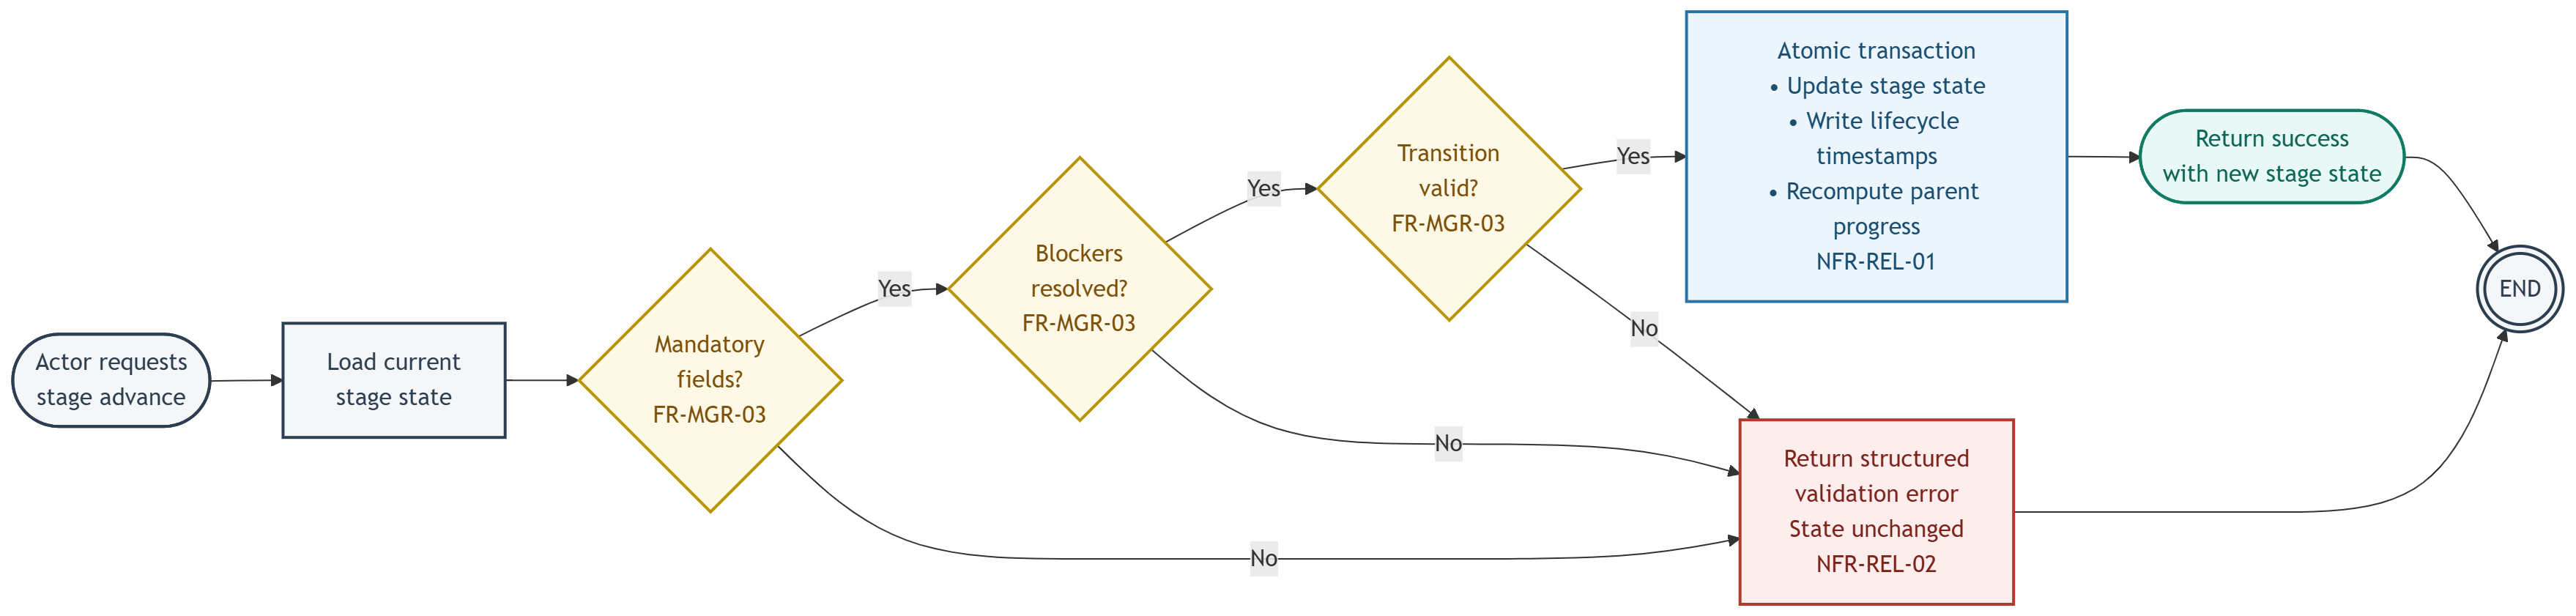
\includegraphics[width=0.85\linewidth,keepaspectratio]{images/fig_3_2_advance_stage.png}%
    }{%
        \fbox{%
            \begin{minipage}[c][6cm][c]{\linewidth}
                \centering
                \textit{[Figure 3.2 placeholder]}
            \end{minipage}%
        }%
    }
    \caption{Activity diagram for \textit{Advance RFQ Stage}}
    \label{fig:activity_advance_stage}
\end{figure}

\subsection{Conversational Flow with the Copilot}
The conversational flow with the copilot is structurally different from the lifecycle workflows of the manager service: a single user turn passes through a sequence of stages, several of which are deterministic policy checks rather than language-model invocations. The detailed per-turn pipeline is developed in Chapter~4 (architecture) and Chapter~5 (implementation) and is not duplicated here.

\section{Methodology}
The methodology that structured this project responds to a
solo-developer constraint with asynchronous interaction between two
supervisors and a remote industrial client. The practices below
preserve engineering rigour within that constraint.

\subsection{Scrumban as the Iteration Framework}
Neither pure Scrum nor pure Kanban fits a single-developer project with asynchronous supervisor and client availability: Scrum's sprint ceremonies are artificial without a team, and Kanban alone lacks the demo cadence that keeps remote stakeholders aligned. \textit{Scrumban} is the hybrid adopted in this project: it retains Scrum's cadence and demo discipline while substituting Kanban-style work-in-progress limits for fixed-length sprints. The Scrumban board follows the six-state workflow of Figure~\ref{fig:scrumban}: \textit{Backlog (Frozen Scope)}, \textit{Ready}, \textit{In Progress}, \textit{Review and Demo}, \textit{Done}, and \textit{Documented}. The terminal \textit{Documented} state treats documentation as part of the definition of done: an item leaves \textit{Done} only when its specification, decision rationale, and validation evidence are written up and committed alongside the code --- the discipline that lets every chapter of this report rest on artifacts produced during implementation rather than reconstructed after the fact.

\begin{figure}[H]
    \centering
    \IfFileExists{images/fig_3_3_scrumban.png}{%
        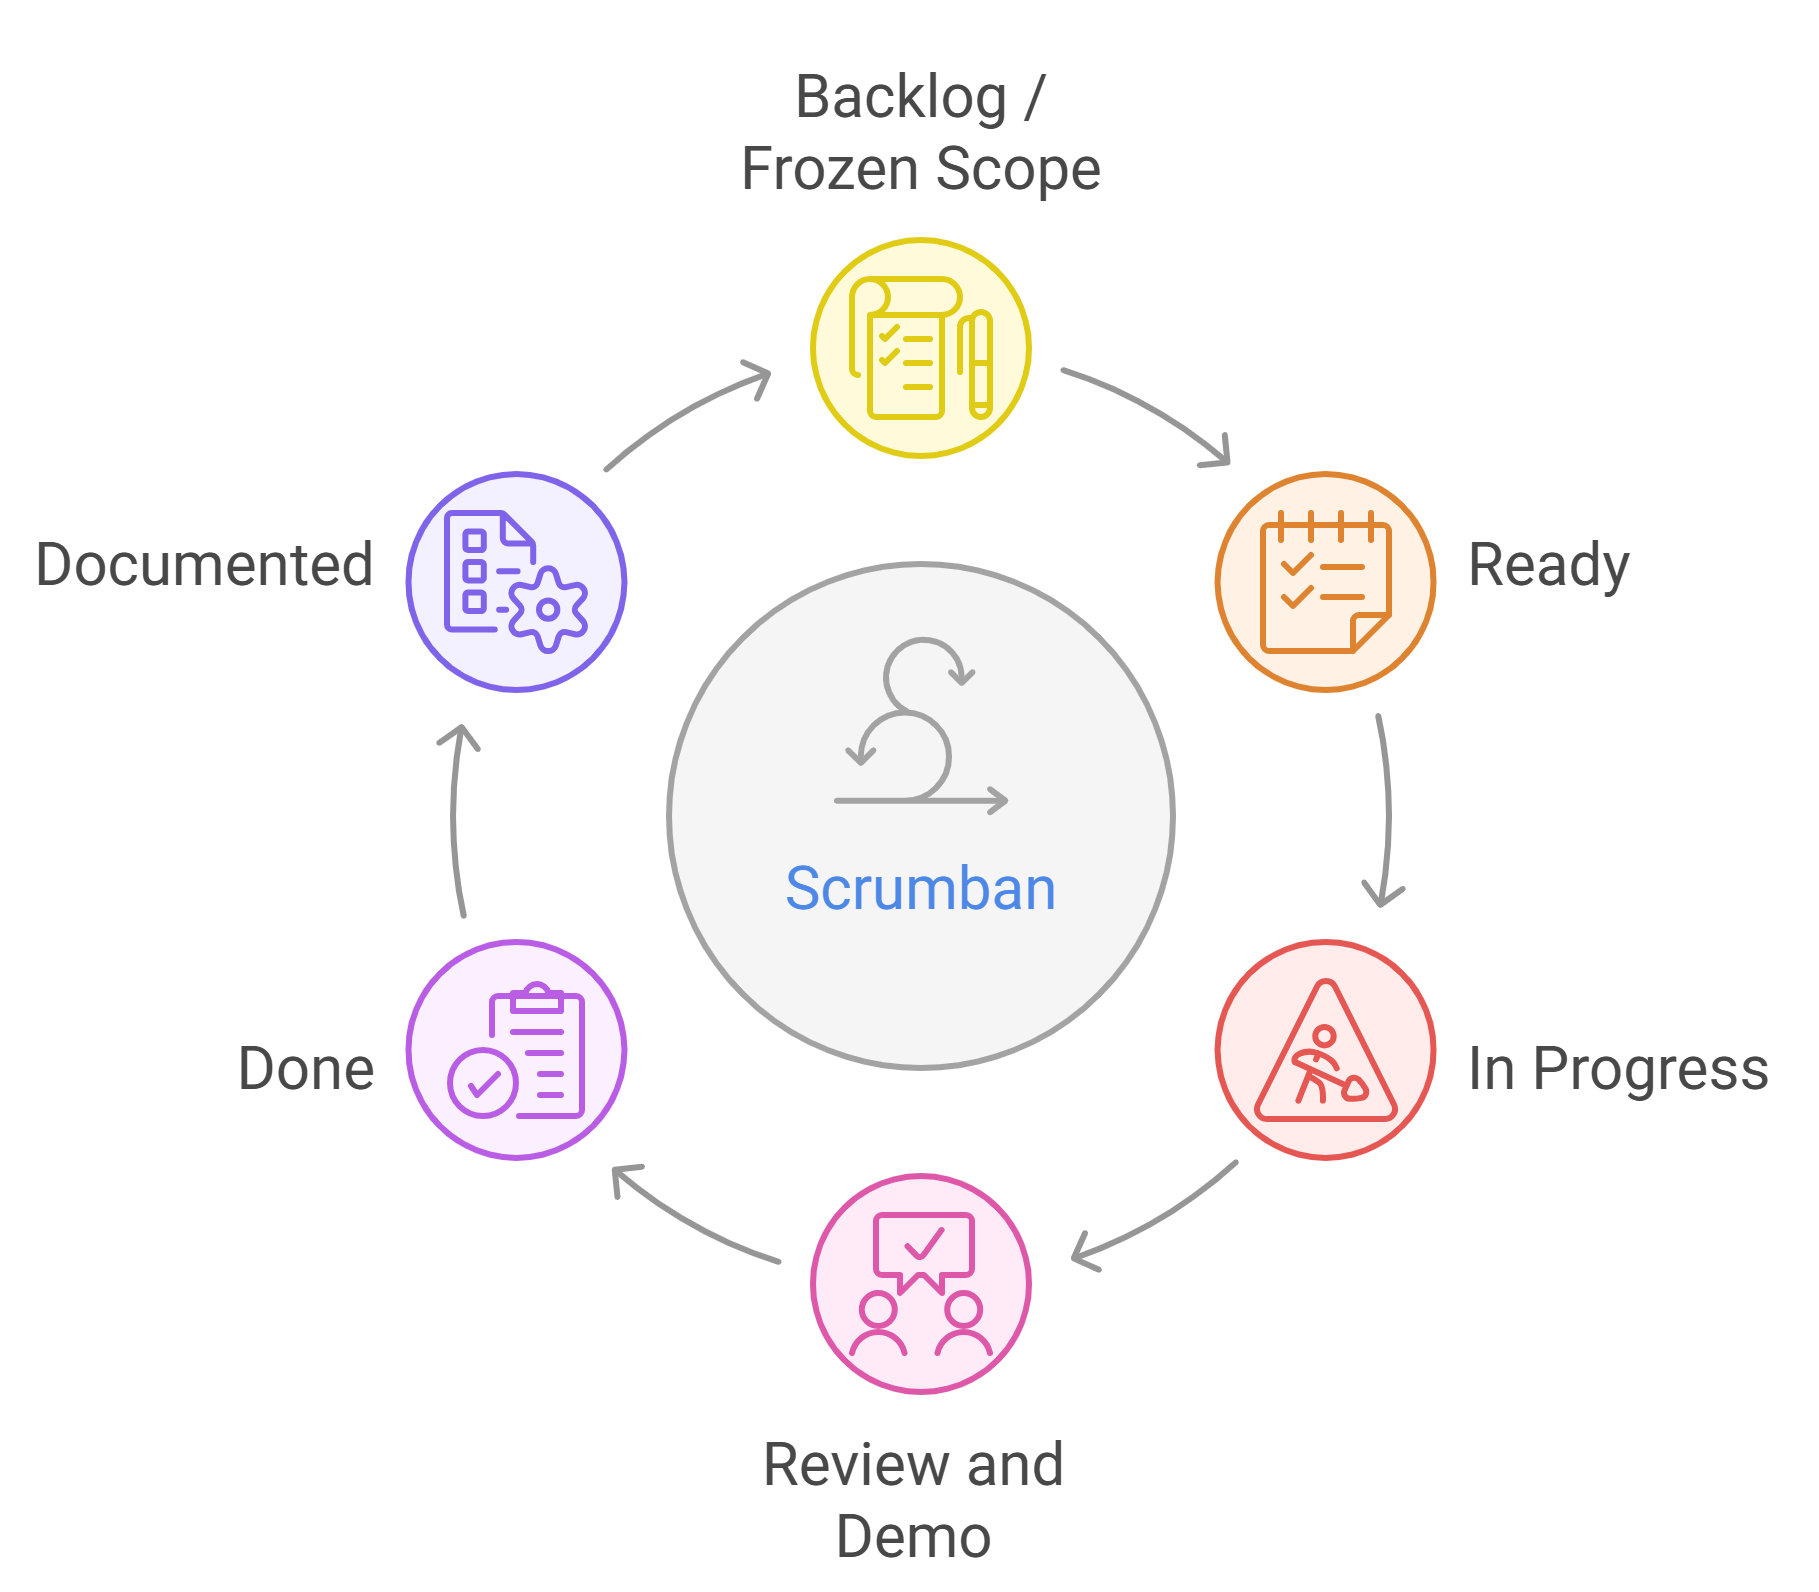
\includegraphics[width=0.85\linewidth,keepaspectratio]{images/fig_3_3_scrumban.png}%
    }{%
        \fbox{%
            \begin{minipage}[c][6cm][c]{\linewidth}
                \centering
                \textit{[Figure 3.3 placeholder]}
            \end{minipage}%
        }%
    }
    \caption{Scrumban six-state workflow board, with \textit{Documented} as the terminal column}
    \label{fig:scrumban}
\end{figure}

\subsection{Architectural Decision Records}
Architectural Decision Records follow a six-part structure: context,
options, decision, justification, consequences, validation. ADR-H5
(\textit{Dormant Models}) is committed to the manager repository as
the fully formalised example; the remaining decisions are documented
in prose in Chapter~4's register, with consolidation into a unified
collection recognised as a hardening direction.

\subsection{Project Control Center}
The Scrumban board, decision register, risk register, and stakeholder
alignment matrix are maintained in a project Control Center built on
Notion, structured as a twelve-section workspace covering scope,
backlog, decisions, risks, stakeholder alignment, and defence
preparation. The Control Center is the single source of truth for
project state throughout the iteration; documents extracted from it
form the basis of this chapter's tables and of the artifacts
referenced throughout the report.

\section*{CONCLUSION}
\addcontentsline{toc}{section}{CONCLUSION}
This chapter has formalised the project's engineering structure: stakeholders and access assumptions, twenty-five functional and nineteen non-functional requirements with explicit scope tags, the use cases and activity diagrams, and the methodology. The next chapter develops the architecture that delivers on this catalogue.